\chapter{基于工具调用路径的工具图谱构建}

\section{引言}

工具调用路径中蕴涵了工具之间的调用关系信息,通过图的格式对工具信息进行建模后,能够通过在图上的搜索来获取工具之间的依赖。
本章介绍了一种基于工具调用路径数据进行工具图谱构造的策略,并基于此方法实现了一个大规模的工具图谱。

本章将会围绕着工具图谱构建中的一些挑战出发,具体来说:
1.如何筛选调用路径数据,得到高质量的工具集以及工具调用路径?
2.如何设计工具图谱的结构,以表示工具之间的依赖关系?
3.如何验证工具图谱作为知识库的有效性?
4.如何有效地在图谱上搜索相关节点?

基于上述问题,我们进行了以下研究:首先,我们提出了三种数据筛选策略,从API工具和API调用路径的角度对数据进行了筛选,保留了一批高质量的工具路径数据。
其次,我们设计了工具动态转移权值和工具静态转移权值两种方式,通过对工具路径数据进行计算,得到了工具之间的转换权值以及每个工具的可用性分数,用于后续辅助大语言模型进行工具选择。
然后,关于验证工具图谱作为知识库的有效性,我们对比了直接用普通的检索增强方式和包含图谱知识的方式,验证了构建工具图谱的有效性和必要性。
最后,我们通过对向量模型进行负样本构造和有监督的微调,获得了一个API检索器,并对工具检索的召回率进行了充分实验,证明了该模型在节点搜索上的有效性。

\section{整体流程}

在现实场景的工具调用场景中,其实不同类型的工具之前存在隐含的顺序关系。举一个现实生活中的例子,“城市经纬度查询”和“根据经纬度获取实时天气”的工具总是在一起使用。
这种存在于工具调用路径中的“过程性知识”对工具规划非常有启发性,能够表示工具之间的调用关系和跳转关系。
基于此,我们希望能够通过对工具之间的转换关系进行建模,并将工具的搜索范围限定在一个更精确的空间,以辅助大语言模型工具调用。

我们分析了目前公开可用的通用工具学习数据集ToolBench、API-Bank,其中包含大量的多跳工具调用路径。通过分析其中的数据,我们发现每个工具后都只有一小部分后继工具会被调用,这证实了我们的观点,即工具之间存在相互调用的关系。

因此我们通过对开源的工具调用路径数据进行数据筛选、数据清洗等流程构建了一个高质量的工具图谱。
数据筛选和清洗流程中,本文制定了根据工具来筛选和根据调用路径筛选两种策略,得到高质量的工具调用路径作为图谱构建的基础数据。
其次,我们设计了知识图谱的本体模型结构,对工具之间的依赖关系进行了建模,将工具数据映射到工具图谱上。
在进行图谱搭建时,我们设计了两种图上的权值:边上的工具转换权值和节点上的工具可用性权值,分别表示工具之间的依赖关系和工具的可用性。并通过图谱构建策略计算出这两个权值和制定了更新策略。
最后,我们根据清洗后的数据和计算得到的工具图边权/点权得到了一个工具图谱,用于指导大语言模型的工具调用,具体使用方法在第四章有详细阐述。

\section{可行性分析}

计算一下每个tool后面跟着的tool的比例(什么的)

\section{数据收集和清洗}

\subsection{数据集介绍}

目前常见的工具调用数据集有ToolBench\cite{Qin2023},EasyTool\cite{yuan2024easytool},API-Bank\cite{Li2023c},TaskBench\cite{shen2023taskbench},ToolAce\cite{liu2024toolace}。

ToolBench主要聚焦的是多情景的工具调用,且使用的是真实世界的API工具,能够通过代码调用,因此本文主要使用的是ToolBench中的数据。

ToolBench包括来自49个类别的16464个真实的RestAPI工具,并根据这些工具构建了包含126486条调用路径的数据集。
ToolBench中使用的API都来自于一个开放的API托管平台“RapidAPI Hub”,在这个API托管平台中包含各种不同类别、不同供应商的API服务,需要订阅了相应的工具集才能够使用。在RapidAPI Hub中,工具以以下的方式进行组织,即网站上有不同的大类,大类下面会有不同的工具集,而工具集下面会有对应的单独的API工具。

ToolBench中包含不同类型的数据,如:1.每个工具集的详细描述信息,包括工具集的名称、描述、类别等 2.工具的输入、输出参数列表 3.工具调用的示例代码 4.工具调用路径

在本文中,为了构建工具图谱,因此我们在图谱构建部分主要利用的是工具调用路径数据。
由于RapidAPI Hub上,同功能的工具可能有很多,
即API工具之间存在着相似性或者能够从功能上相互替换,
因此对于同一个用户任务,有多条路径都能够解决问题。
因此对于每个需求,并不存在一个标准答案路径。
但是我们可以通过分析最终的回答结果,
判断经过一组API顺序调用之后系统输出的结果是否符合预期,
来判断路径是否合理。

\subsection{数据清洗}

\subsubsection{工具节点筛选}

在筛选高质量API工具之前,我们首先限定了工具的应用领域,聚焦于购物、旅游、天气和餐饮四个类别。这些类别的API工具功能丰富,为用户提供了广泛的应用场景支持。

在工具的初步筛选后,我们对API的描述信息丰富度进行了严格评估和筛选。为此,我们使用了大语言模型进行批量打分,并设计了一套评分标准来量化描述信息的质量,从三个维度进行评估:描述的完整性(如是否详细说明功能)、易读性(如是否语义清晰)。

每个维度的分数范围为1到3分,其中:
\begin{itemize}
    \item 1分:不满足要求;
    \item 2分:基本满足要求,但有一定的不清晰或者不完整;
    \item 3分:描述非常详细,语言清晰流畅,信息完整且丰富。
\end{itemize}

筛选规则为:只有在所有维度上均得分为3分的工具才会被保留下来。

为验证大语言模型的打分可靠性,我们抽样了100个API的信息提交给3位人工评审员进行独立打分,并与大语言模型的打分结果进行了对比分析。

一致性(Consistency)在此处定义为人工打分与大语言模型打分结果的完全一致性。如果人工评审员与大语言模型对同一API的打分在某一维度上相同,则认为该API在该维度的评分是一致的。表中的一致性百分比是根据以下公式计算的:

\[
\text{一致性 (\%)} = \frac{\text{人工与大模型打分相同的API数量}}{\text{总API数量}} \times 100
\]

该指标用于量化大语言模型评分与人工评审之间的匹配程度,从而验证模型评分的可靠性。

表\ref{tab:api_score_comparison}展示了两者在不同维度下的评分分布及一致性。

\begin{table}[h]
  \centering
  \caption{Comparison of Human and Model Scoring Distribution}
  \label{tab:api_score_comparison}
  \begin{tabular}{l|c|c|c}
  \toprule
  \textbf{Dimension} & \textbf{Score} & \textbf{Human Count} & \textbf{Model Count} \\ \midrule
  \multirow{3}{*}{Completeness} & 1 & 20 & 22 \\ 
                                & 2 & 40 & 38 \\ 
                                & 3 & 40 & 40 \\ \hline
  \textbf{Completeness Consistency} & \multicolumn{3}{c}{84\%} \\ \midrule
  \multirow{3}{*}{Readability}  & 1 & 18 & 20 \\ 
                                & 2 & 42 & 40 \\ 
                                & 3 & 40 & 40 \\ \hline
  \textbf{Readability Consistency} & \multicolumn{3}{c}{79\%} \\ 
  \bottomrule
  \end{tabular}
  \end{table}

由上可见,人工打分与大语言模型打分具有较高的一致性,说明大语言模型评分与人工评审具有较高的可信度。


在完成描述信息筛选后,我们对筛选出的API进行了连通性测试,以确保其实际可用性。测试内容包括:
\begin{itemize}
    \item 响应状态码;
    \item 请求响应时间;
    \item 错误信息;
    \item 返回内容的完整性。
\end{itemize}

最终,仅保留响应状态码为正常且在规定时间内返回有效内容的API工具。

通过筛选,我们从初始的工具池中提取了\textbf{150个高质量API工具},这些工具在描述信息和功能性两方面均表现优异,涵盖购物、旅游、天气和餐饮四个领域。
筛选后的API工具分布情况如下:

\begin{table}[h]
  \centering
  \caption{Distribution of API tools by category after filtering}
  \label{tab:api_distribution}
  \begin{tabular}{l|c|c}
  \toprule
  \textbf{Category} & \textbf{Number of Tools} & \textbf{Number of APIs} \\ \midrule
  Shopping & 18 & 40 \\ \hline
  Travel   & 22 & 50 \\ \hline
  Weather  & 15 & 45 \\ \hline
  Dining   & 10 & 25 \\ 
  \bottomrule
  \end{tabular}
  \end{table}

\subsubsection{工具调用路径筛选}

工具调用路径数据可能会有未完成任务导致失败/工具调用出错等问题,
并且数据集中的工具调用是以决策树的方式组织的,需要从中进行剪枝获得正确的线性的工具路径。
基于上述问题,我们对工具调用路径数据进行了一些清洗,主要筛选方式如下:

\textbf{删除失败任务}:为确保工具调用路径能准确解答用户需求,我们仅保留成功调用并产生结果的工具调用路径,删除那些无法得出有效结果的工具调用决策树。具体依据调用路径中的 \texttt{"finish\_type"} 字段进行筛选,其中 \texttt{"give\_answer"} 的路径保留,\texttt{"give\_up"} 的路径丢弃。

\textbf{对工具调用树进行剪枝}:在ToolBench中的工具调用树中,工具的探索和调用路径是以决策树的形式组织的,因此我们需要对工具调用树进行剪枝,以获得一条线性的工具调用路径。因此,我们通过数据中的 \texttt{"pruned"} 字段进行剪枝,仅保留 \texttt{"pruned"} 为 \texttt{"false"}的字段。

\textbf{删除调用错误节点}:在筛选优质工具路径后,我们需要进一步清洗工具路径数据,以确保调用路径上的工具都可执行。我们在调用路径中根据\texttt{"error"}字段的内容来决定是否删除节点。对于调用过程中发生错误的工具节点(如未授权错误、API不可用等错误),将其从路径中剔除,以确保路径的完整性和可执行性。最终,保留下的应该是一条线性且无错误的调用路径。

% \begin{table}[h!]
%   \centering
%   \begin{tabular}{|l|p{10cm}|} % 第二列设置为宽度为 10cm 的段落列
%   \hline
%   \textbf{Error Type} & \textbf{Description} \\ \hline
%   API Not Working Error (Unreachable) & The API server is not reachable, possibly due to server downtime or network issues. \\ \hline
%   Message Error & The response message has a formatting issue or cannot be parsed correctly. \\ \hline
%   Timeout Error & The request to the API timed out due to slow response or network delays. \\ \hline
%   Request Invalid, Data Error & The request contains invalid parameters, incorrect data, or violates API rules. \\ \hline
%   Unauthorized Error & The client does not have the required permissions or valid credentials to access the API. \\ \hline
%   \end{tabular}
%   \caption{API Error Types and Their Descriptions}
%   \label{tab:api_errors}
% \end{table}


% 【最好画一个图,表示三种数据筛选的逻辑】

% 原始数据集中包含了xx条工具调用路径数据,
% 其中平均的工具调用次数为xxx次,
% 经过上述的筛选逻辑后,共剩下xxx条工具调用路径数据,平均工具调用次数为xx次,
% 我们基于该高质量的路径数据集建立工具图谱。

% 工具图谱的构建对于系统整体的性能和效率至关重要。
% 在这里,我们参考了ToolNet\cite{Liu2024}中的设计,
% 将API工具作为图谱中的工具节点,
% 工具节点之间的边上带有一个权值,该权值叫做“工具转移权值”,用于代表
% 从当前工具出发,有多大的可能性会跳转到调用另一个工具的使用。
% 除了边上带有权值,我们给工具节点也赋予了一个权值,该权值叫做“工具可用性权值”,用于表示该
% 工具的可用性。因此,在该工具图谱中,权值的计算方式非常重要。边和点的权值应该有区分度,不然无法提供有效的信息。

% 我们首先将会介绍基于历史工具调用数据的静态图谱构建方式,由于API工具具有时效性和多变性,我们还会对图上的节点、节点权值还有边上的权值进行动态的更新。


\section{图谱构建}

\subsection{工具图谱概念模型}

工具图谱中的实体类别主要包括三种:工具节点、工具组节点和工具类别节点。每种实体类别分别表示不同的抽象层次和功能,具体如下:

\subsubsection{工具(Tool)}
工具节点是图谱的基础实体,表示具体的API接口工具或单个功能模块。其属性如下:
\begin{itemize}
    \item \textbf{Name(名称)}:工具的唯一标识名称。
    \item \textbf{URL(接口地址)}:API工具的访问地址。
    \item \textbf{Description(描述)}:工具的简要说明,通常用于描述其用途或功能。
    \item \textbf{Method(请求方法)}:支持的HTTP方法,如GET、POST等。
    \item \textbf{Required Parameters(必需参数)}:调用API所需的必填参数列表。
    \item \textbf{Optional Parameters(可选参数)}:调用API的可选参数列表。
    \item \textbf{Test Endpoint(测试端点)}:用于测试的API地址或信息。
\end{itemize}

在工具图谱的组织中,每个工具节点只属于一个工具组。多个工具可以归属于同一个工具组,从而形成对工具功能的逻辑分类。例如,“酒店搜索”工具和“酒店评论查询”工具都可能属于“旅游服务工具组”。这种一对多的归属关系确保工具图谱结构的清晰性,同时避免工具节点的多重归属问题。

\subsubsection{工具组(Tool Group)}
工具组节点表示一组功能相关的工具的集合,用于组织和分类多个工具节点。其属性如下:
\begin{itemize}
    \item \textbf{Product ID(产品ID)}:工具组的唯一标识符。
    \item \textbf{Tool Description(工具描述)}:对该工具组的整体描述。
    \item \textbf{Home URL(链接)}:工具组的官网链接或信息页面。
    \item \textbf{Name(名称)}:工具组的名称。
    \item \textbf{Title(标题)}:工具组的显示标题。
    \item \textbf{Pricing(定价)}:工具组的定价信息,例如``免费(FREE)''。
    \item \textbf{Tool Name(工具名称)}:与工具组相关联的主要工具名称。
    \item \textbf{Score(评分)}:工具组的相关指标,包括:
        \begin{itemize}
            \item \textbf{AvgServiceLevel(服务水平平均值)}:表示服务稳定性的指标,百分比表示。
            \item \textbf{AvgLatency(平均延迟)}:工具组调用的平均延迟时间,单位为毫秒。
            \item \textbf{AvgSuccessRate(成功率平均值)}:表示API调用成功率的平均值,百分比表示。
            \item \textbf{PopularityScore(流行度评分)}:工具组的受欢迎程度评分。
        \end{itemize}
    \item \textbf{Host(请求地址)}:工具组所关联的主要域名地址。
\end{itemize}

工具组进一步与工具类别关联,每个工具组只属于一个工具类别,从而实现高层次的分类。例如,“旅游服务工具组”可以归属于“旅游与出行”类别。工具组与工具类别之间的一对多关系,能够有效区分不同工具组的功能领域。


\subsubsection{工具类别(Tool Category)}
工具类别节点表示工具所属的领域、用途或分类。例如,工具类别可以表示工具的主要负责内容为“旅游出行”、“美食”或“电影媒体”。其属性如下:
\begin{itemize}
    \item \textbf{Name(名称)}:类别的名称,用于标识该类别。
    \item \textbf{Description(描述)}:对工具类别的简要说明,描述其应用场景或技术范围。
\end{itemize}

工具类别节点与工具组节点的关系是唯一的映射关系,每个工具组只能归属于一个工具类别。此外,工具节点的类别由其所属工具组的类别决定,工具节点和工具组的类别在逻辑上保持一致。这种设计保证了工具图谱的分类层次统一性。例如,“酒店搜索”工具属于“旅游服务工具组”,“旅游服务工具组”属于“旅游与出行”类别,因此“酒店搜索”工具的类别也是“旅游与出行”。


工具之间的依赖关系通常分为三种\cite{shen2023taskbench}:时序依赖、资源依赖、环境依赖。
环境依赖指工具运行所需的外部环境条件(如特定硬件、操作系统或软件版本等)。在本研究中,由于工具多为基于REST API的服务接口,不涉及环境依赖。
因此,本文在工具图谱构建中仅考虑时序依赖和资源依赖两种依赖关系。

在工具图谱的概念模型中,依赖关系主要包括以下三种类型:

\subsubsection{时序依赖(Sequential Dependency)}
时序依赖指的是在历史工具调用路径中被连续调用的两个工具之间的关系。描述如下:
\begin{itemize}
    \item \textbf{起点(Source)}:工具A。
    \item \textbf{终点(Target)}:工具B。
    \item \textbf{关系描述(Description)}:工具B在调用时需要工具A的先行调用。
\end{itemize}

\subsubsection{强资源依赖(Strong Resource Dependency)}
强资源依赖指的是某种资源或信息仅能通过前一个工具获取,然后提供给后一个工具。例如,一个旅行商的“酒店ID搜索”工具获取特定的酒店ID,而“酒店评论搜索”工具必须依赖该ID。描述如下:
\begin{itemize}
    \item \textbf{起点(Source)}:工具A。
    \item \textbf{终点(Target)}:工具B。
    \item \textbf{资源类型(Resource Type)}:强依赖的资源类型,例如``酒店ID''。
    \item \textbf{关系描述(Description)}:工具A输出的资源是工具B必须依赖的输入。
\end{itemize}

\subsubsection{弱资源依赖(Weak Resource Dependency)}
弱资源依赖指的是某种资源或信息可以通过另一个工具获取,但不是必须的。例如,“根据经纬度搜索降雨情况”工具可以直接调用,也可以通过“城市经纬度搜索”工具提供经纬度作为输入。描述如下:
\begin{itemize}
    \item \textbf{起点(Source)}:工具A。
    \item \textbf{终点(Target)}:工具B。
    \item \textbf{资源类型(Resource Type)}:弱依赖的资源类型,例如``经纬度''。
    \item \textbf{关系描述(Description)}:工具B的输入可以由工具A提供,但也可以通过其他方式获取。
\end{itemize}

\subsection{实例模型构建}

本节详细阐述工具知识图谱的构建过程,包括节点和依赖关系的抽取、存储,以及如何将数据导入Neo4j进行存储和查询。同时探讨如何扩展图谱构建的内容和方法,为更丰富的应用场景提供支持。

\subsubsection{直接用规则抽取所有工具组、工具、类别节点}

工具组、工具和工具类别节点的抽取主要依赖规则匹配。从现有的JSON格式工具描述文档中,按照预定义规则通过代码匹配关键信息。工具组的抽取字段包括产品ID、工具组名称、工具组描述和主页链接等信息,这些字段为工具组提供全局标识及其关联性。工具节点的提取则更加具体,记录每个工具的名称、API地址、功能描述、HTTP方法(如GET或POST)、必需参数和可选参数等关键信息。工具类别节点用于标识技术领域或功能分类,从技术标签中提取类别名称、描述及相关技术栈等字段。

通过规则提取的节点数据存储为结构化格式。这些文件为图谱数据导入提供了清晰的数据基础,确保后续步骤的顺利进行。

\subsubsection{直接用代码规则抽取时序依赖}

时序依赖是通过分析工具调用日志数据来构建的。首先,对调用日志按照时间戳进行排序,从而生成工具调用的顺序链条。接着,识别这些调用链中的连续工具对,将其标记为时序依赖。这种依赖通常用于捕获工具在真实调用路径中的关系,反映调用流程的顺序逻辑。例如,旅行工具链中“酒店搜索”紧接着“酒店评论查询”,这反映了用户实际使用时的时序逻辑。

抽取后的时序依赖关系记录起点工具、终点工具、依赖类型(标记为“时序依赖”)以及描述字段。时序依赖的记录不仅有助于绘制工具调用路径,还为分析流程优化提供依据。

\subsubsection{规则+大语言模型的依赖构建}

在资源依赖关系的构建中,规则匹配与大语言模型(LLM)结合的方式被应用。首先,通过规则匹配提取工具的输入参数和输出字段,将字段名和类别进行对比,初步判断是否存在资源依赖。例如,“酒店评论查询”工具需要“酒店ID”作为输入,如果“酒店ID”是由“酒店搜索”工具提供的输出,则可以标记为强依赖关系。规则匹配能够高效处理结构化和模式化的依赖,但在复杂场景下可能有所不足。

对于规则匹配识别出的潜在依赖关系,大语言模型进一步进行验证和分类。通过将两个工具的API文档(包括功能描述、输入和输出定义等)传递给模型,询问是否存在依赖关系,并让模型判断依赖关系的类型(强依赖或弱依赖)及其依赖字段。例如,大语言模型可能识别“根据经纬度查询天气”工具对“城市经纬度搜索”工具的弱依赖关系,说明输入经纬度可以通过其他手段获取但更倾向于使用特定工具。识别完成后,依赖关系被整理为规范化的数据格式,方便导入图谱中。

\subsubsection{图谱数据导入}

构建完成的工具知识图谱数据需要导入Neo4j图数据库,以支持高效存储和复杂查询。数据导入分为节点和关系两部分。首先,工具、工具组和工具类别被转化为图中的节点。它们分别通过名称、ID等标识字段建立类型,并与属性字段一一关联。

关系数据的导入使用工具节点的标识字段建立工具之间的依赖关系,包括时序依赖、强资源依赖和弱资源依赖。依赖关系被标注有明确的类型和描述字段,便于在查询中准确反映其性质。导入完成后,可以通过可视化工具验证图谱中的节点和关系,确保结构的准确性和逻辑性。

【可视化的一个图,Neo4j的截图】

% \begin{itemize}
%   \item 时序依赖:时序依赖指的是在历史工具调用路径中被连续调用的两个工具。
%   \item 强资源依赖:在资源依赖部分,我们根据资源的强弱依赖进行区分。强依赖指的是某种资源/信息仅能通过前一个API工具获取,然后提供给后一个API工具。比如某个旅行商有自己设定的酒店ID,而搜索酒店评论时必须根据该ID来获取,那么在“酒店ID搜索”和“酒店评论搜索”两个工具之间就存在“酒店ID”的强依赖关系。
%   \item 弱资源依赖:弱资源依赖指的是API工具的某种资源/信息可以通过另一个API工具获取,但是不是必须的。比如我们要搜索“根据经纬度搜索降雨情况“时,首先需要获取上海的经纬度。这个经纬度既可以通过大语言模型本身的知识获取,也可以通过”城市经纬度搜索“工具来获取。因此这种资源依赖关系不是必须的,而是可以通过大语言模型、多个API工具提供。
% \end{itemize}


% \subsection{静态构建}

% 静态构建图的过程相对简单,只需要遍历路径数据,并计算每两个节点之间的边权和点权值即可。

% 设定 $D$ 为已完成任务的工具使用路径集合,每条路径由工具使用的顺序构成,

% \[
% \text{Trajectory} = [D_1, D_2, \ldots, D_n]
% \]

% 假设每个工具的调用成功与否是一个二元变量 $x_i$,其中:

% \[
% x_i = 
% \begin{cases} 
% 1, & \text{工具调用成功} \\
% -1, & \text{工具调用失败}
% \end{cases}
% \]

% 为了简化操作,我们将“结束”视为一种普通工具,每个工具都与“结束”工具节点相连,
% 当大语言模型智能体认为要结束调用过程时,就会选择“结束”工具。

% 节点 $v_i$ 到 $v_j$ 的转移权重 $w_{i,j}$ 计算如下:

% \[
% w_{i,j} = \frac{\mathbb{E}_D[1(\text{tool}_s = v_i \land \text{tool}_{s+1} = v_j)]}{\mathbb{E}_D[1(\text{tool}_s = v_i)]}
% \]

% 其中,$\mathbb{E}_D[\cdot]$ 表示对路径集合 $D$ 上的期望操作,$1(\cdot)$ 是指示函数,当条件满足时取值为1,否则为0。
% 该公式计算了工具 $v_i$ 被调用后紧接着调用工具 $v_j$ 的频率。

% 除了关注工具之间的依赖关系,每个单独的工具的可用性和稳定性也是真实场景下重要考虑因素。
% 在工具调用路径中,有一些工具调用会出现无访问权限或访问超时的错误信息。
% 因此我们在工具图中通过对节点的权值进行计算和定义,通过点权来表示该工具的可用性或稳定性。
% 节点 $v_i$ 的可用性权重 $\alpha_i$ 计算如下:

% \[
% \alpha_i = \frac{\sum_{s=1}^{n} 1(x_s = 1 \land \text{tool}_s = v_i)}{\sum_{s=1}^{n} 1(\text{tool}_s = v_i)} \quad (0 \leq \alpha_i \leq 1)
% \]

% 这里,$\alpha_i$ 表示工具 $v_i$ 的调用成功率,是该工具在路径中成功调用的次数与其总调用次数的比值。
% 因此该权值的范围是0-1,越接近1,表示该工具的可用性越高,越接近0,表示该工具的可用性越低。

% \subsubsection{分数映射函数}

% 函数 $f(x)$ 用于将累积分数映射到 $(0, +\infty)$ 的范围内,从而确保在权重更新过程中生成正值。归一化的必要性在于,它能够确保所有工具的表现有效比较,避免负值对权重更新造成不良影响。具体而言,映射函数确保所有工具的权重更新结果均为正值,这对于构建有效的工具图谱至关重要。同时,函数通过灵活处理正负分数,使算法在不同情境下保持良好表现,保持各工具之间的相对表现,从而提升模型的准确性和稳定性。函数定义如下:

% \[
% f(x) :=
% \begin{cases}
% \alpha x + 1, & \text{if } x \geq 0 \\
% e^{\alpha x}, & \text{if } x < 0
% \end{cases}
% \]

% 在这个函数中,$\alpha$ 是控制映射函数行为的超参数。对于正分数,映射为线性函数 $f(x) = \alpha x + 1$,使得得分的正向提升以线性方式反映在权重更新中。对于负分数,映射为指数衰减函数 $f(x) = e^{\alpha x}$,这保证了即使在评分较低的情况下,权重的更新也会保持在一个合理的范围内。

% 通过对筛选后的工具路径数据进行上述计算,我们得到了工具图谱的初始静态图谱。

% \subsection{动态更新}

% 基于上述方法构建的静态工具图谱,本文还提出了对边权和点权的动态更新。
% 动态更新对于工具图谱的构建至关重要,原因主要包括以下几点:
% \begin{itemize}
%   \item \textbf{用户偏好的动态变化}:在实际应用中,随着用户行为的变化,新的调用路径会不断生成。这些新路径反映了用户的真实偏好,因此需要及时添加到工具图谱中,使其能够反映最新的用户需求。
%   \item \textbf{工具的生命周期变化}:工具是动态变化的,随着时间推移,有些工具可能会因为开发者的弃用或其他原因而逐渐失去支持。静态构建无法反映这些变化,而需要通过动态更新来调整图中的边权重,确保图谱能够保持对工具现状的准确表示。
% \end{itemize}

% 动态更新发生的时间节点为系统产生了新的工具调用路径时。

% 以下是对于边权和点权更新的具体阐述,以及对保持分数为正的映射函数的介绍。

% \subsubsection{边权的动态更新}

% 对图 \( G \) 的更新尤为关键。由于可用工具路径的数量有限,我们需要对每一条路径进行细致检查。
% LLM 作为工具的评估者,将整个路径作为输入,评估每个工具节点的表现。

% 我们用 \( \Delta_i^{(n)} \) 表示在第 \( n \) 次迭代中节点 \( v_i \) 的评估得分。
% 节点 \( v_i \) 的累积得分 \( s_i^{(n)} \) 计算如下:

% \[
% s_i^{(n)} = \sum_{k=1}^{n} \Delta_i^{(k)}
% \]

% 该公式对节点 \( v_i \) 在每次迭代中的评分进行累积,为后续的转移权重更新提供基础。

% 节点 \( v_i \) 到 \( v_j \) 的转移权重 \( w_{i,j}^{(n)} \) 在第 \( n \) 次迭代中的更新公式如下:

% \[
% w_{i,j}^{(n)} = \beta w_{i,j}^{(0)} + (1 - \beta) \Delta w_{i,j}^{(n)}
% \]

% 其中,\( w_{i,j}^{(0)} \) 是初始的转移权重,\( \beta \) 是控制初始权重与动态更新之间平衡的超参数,\( \Delta w_{i,j}^{(n)} \) 是用于更新转移权重的归一化梯度,计算公式如下:

% \[
% \Delta w_{i,j}^{(n)} = \frac{f(s_i^{(n)})}{\sum_{v_j \in \text{oneigh}(v_i)} f(s_j^{(n)})}
% \]

% 该公式通过累积分数 \( s_i^{(n)} \) 和 \( s_j^{(n)} \) 来更新转移权重,确保工具之间的转移反映最新的评估结果。

% \subsubsection{点权的动态更新}

% 在点权的动态更新中,我们通过分析新生成的工具调用路径来调整工具的可用性权重。设调用路径为:

% \[
% \text{Trajectory} = [D_1, D_2, \ldots, D_n]
% \]

% 对于每个工具 \( D_i \) 的调用结果记作 \( x_i \),其中:

% - \( x_i = -1 \) 表示调用出错,
% - \( x_i = +1 \) 表示调用成功。

% 在这里,出错的调用情况指的是 API 工具本身存在可用性问题,例如遇到状态码“403 Forbidden”、“408 Request Timeout”等。

% 根据调用结果,我们可以对点权的分数进行更新。更新公式如下:

% \[
% v_i^{(n)} = \beta v_i^{(0)} + (1 - \beta) \Delta v_i^{(n)}
% \]

% 其中:
% - \( v_i^{(0)} \) 是工具 \( D_i \) 的初始权重,
% - \( \beta \) 是控制初始权重与动态更新之间平衡的超参数,其值会根据错误信息的严重程度进行调整,
% - \( \Delta v_i^{(n)} \) 是用于更新权重的归一化梯度,计算公式如下:

% \[
% \Delta v_i^{(n)} = \frac{f(s_i^{(n)})}{\sum_{D_j \in \text{oneigh}(D_i)} f(s_j^{(n)})}
% \]

% 在此公式中,$f(s_i^{(n)})$ 是累积分数,通过反映工具 \( D_i \) 的评估结果,确保工具之间的转移权重反映最新的使用情况和反馈。

% \subsection{图谱数据导入}

% 通过上述操作,我们已经得到了构建工具图谱的原始数据,接下来我们需要将改数据转为供Neo4j存储的图谱数据。具体实现如下所示:



% \section{插图}

% 插图功能是利用 \TeX{} 的特定编译程序提供的机制实现的,不同的编译程序支持不同的图
% 形方式。有的同学可能听说“\LaTeX{} 只支持 EPS”,事实上这种说法是不准确的。\XeTeX{}
% 可以很方便地插入 EPS、PDF、PNG、JPEG 格式的图片。

% 一般图形都是处在浮动环境中。之所以称为浮动是指最终排版效果图形的位置不一定与源文
% 件中的位置对应,这也是刚使用 \LaTeX{} 同学可能遇到的问题。如果要强制固定浮动图形
% 的位置,请使用 \pkg{float} 宏包,它提供了 \texttt{[H]} 参数。

% \subsection{单个图形}

% 图要有图题,研究生图题采用中英文对照,并置于图的编号之后,图的编号和图题应置于图
% 下方的居中位置。引用图应在图题右上角标出文献来源。文中必须有关于本插图的提示,如
% “见图~\ref{fig:energy-distrib}”、“如图~\ref{fig:energy-distrib} 所示”等。该页空
% 白不够排写该图整体时,则可将其后文字部分提前排写,将图移到次页。

% \begin{figure}[!htp]
%   \centering
%   \begin{tikzpicture}
%     \begin{axis}[
%       width=12cm,
%       height=9cm,
%       xmin=0, xmax=7,
%       xlabel={$r$ (\unit{\milli\metre})},
%       ymin=-1000, ymax=11000,
%       ylabel={Energy (\unit[per-mode=symbol]{\watt\per\cubic\metre})},
%       scaled ticks=false,
%       tick label style={
%         /pgf/number format/1000 sep=,
%         font={\zihao{-5}},
%       },
%       minor tick num=1,
%       tick pos=left,
%       tick align=outside,
%       tick style={thin,black},
%     ]
%       \addplot [only marks,mark=square*] 
%         table [x={radial}, y={energy}, col sep=comma] 
%         {./assets/energy-distrib.csv};
%       \node at (2,6000) 
%         {$q_{v}=\dfrac{\sigma\omega^{2}|\mathbf{A}|^{2}}{2}$};
%     \end{axis}
%   \end{tikzpicture}
%   \bicaption{内热源沿径向的分布}{Energy distribution along radial}
%   \label{fig:energy-distrib}
% \end{figure}

% \subsection{多个图形}

% 简单插入多个图形的例子如图~\ref{fig:SRR} 所示。这两个水平并列放置的子图共用一个
% 图形计数器,没有各自的子图题。

% \begin{figure}[!htp]
%   \centering
%   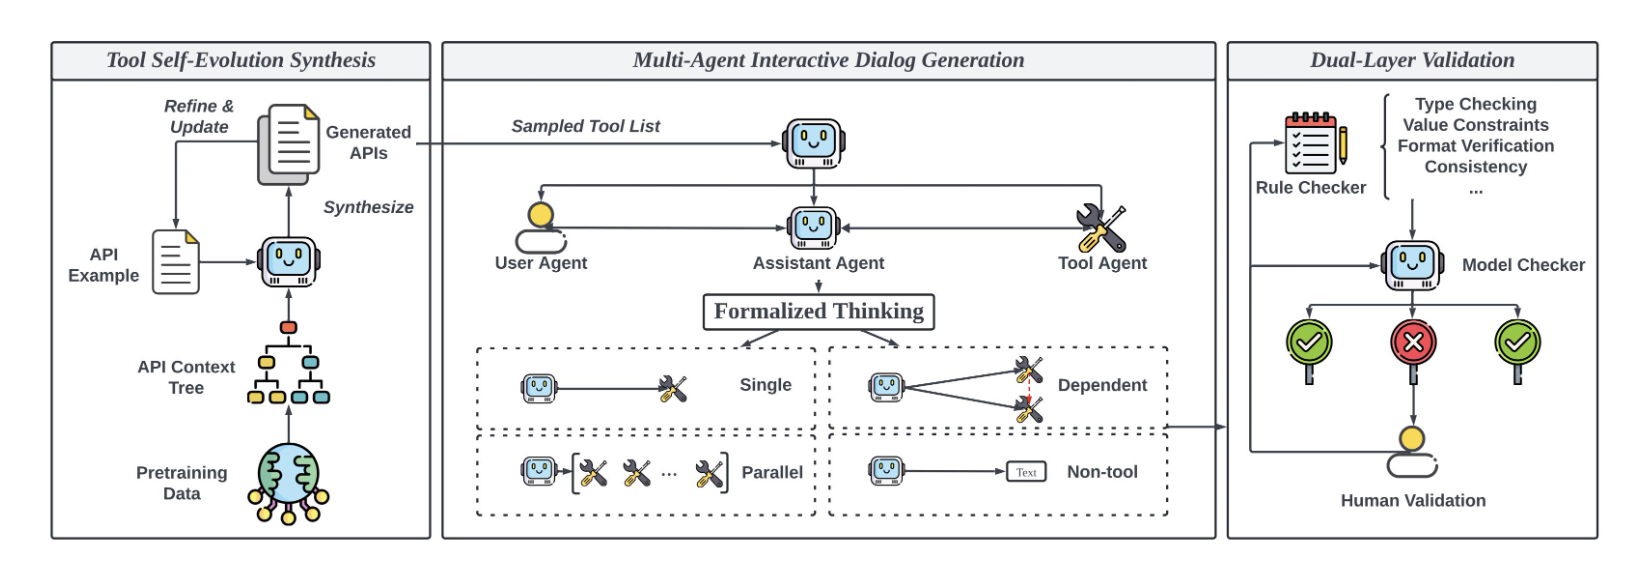
\includegraphics[height=2cm]{../assets/1.png}
%   \hspace{1cm}
%   \includegraphics[height=2cm]{sjtu-vi-badge-red.pdf}
%   \bicaption{中文题图}{English caption}
%   \label{fig:SRR}
% \end{figure}

% 如果多个图形相互独立,并不共用一个图形计数器,那么用 \texttt{minipage} 或者
% \texttt{parbox} 就可以,如图~\ref{fig:parallel1} 与图~\ref{fig:parallel2}。

% \begin{figure}[!htp]
%   \centering
%   \begin{minipage}{0.48\textwidth}
%     \centering
%     \includegraphics[height=1.7cm]{sjtu-vi-name-red.pdf}
%     \caption{并排第一个图}
%     \label{fig:parallel1}
%   \end{minipage}\hfill
%   \begin{minipage}{0.48\textwidth}
%     \centering
%     \includegraphics[height=1.7cm]{sjtu-vi-name-red.pdf}
%     \caption{并排第二个图}
%     \label{fig:parallel2}
%   \end{minipage}
% \end{figure}

% 如果要为共用一个计数器的多个子图添加子图题,建议使用较新的 \pkg{subcaption} 宏
% 包,不建议使用 \pkg{subfigure} 或 \pkg{subfig} 等宏包。

% 推荐使用 \pkg{subcaption} 宏包的 \cs{subcaptionbox} 并排子图,子图题置于子图之
% 下,子图号用 a)、b) 等表示。也可以使用 \pkg{subcaption} 宏包的 \cs{subcaption}
% (放在 minipage中,用法同 \cs{caption})。

% \pkg{subcaption} 宏包也提供了 \pkg{subfigure} 和 \pkg{subtable} 环境,如
% 图~\ref{fig:subfigure}。

% \begin{figure}[!htp]
%   \centering
%   \begin{subfigure}{0.3\textwidth}
%     \centering
%     \includegraphics[height=2cm]{sjtu-vi-badge-red.pdf}
%     \caption{校徽}
%   \end{subfigure}
%   \hspace{1cm}
%   \begin{subfigure}{0.4\textwidth}
%     \centering
%     \includegraphics[height=1.7cm]{sjtu-vi-name-red.pdf}
%     \caption{校名。注意这个图略矮些,subfigure 中同一行的子图在顶端对齐。}
%   \end{subfigure}
%   \caption{包含子图题的范例(使用 subfigure)}
%   \label{fig:subfigure}
% \end{figure}

% 搭配 \pkg{bicaption} 宏包时,可以启用 \cs{subcaptionbox} 和 \cs{subcaption} 的双
% 语变种 \cs{bisubcaptionbox} 和 \cs{bisubcaption},如图~\ref{fig:bisubcaptionbox}
% 所示。

% \begin{figure}[!hbtp]
%   \centering
%   \bisubcaptionbox{$R_3 = 1.5\text{mm}$ 时轴承的压力分布云图}%
%                   {Pressure contour of bearing when $R_3 = 1.5\text{mm}$}%
%                   [6.4cm]{\includegraphics[height=3cm]{example-image-a.pdf}}
%   \hspace{1cm}
%   \bisubcaptionbox{$R_3 = 2.5\text{mm}$ 时轴承的压力分布云图}%
%                   {Pressure contour of bearing when $R_3 = 2.5\text{mm}$}%
%                   [6.4cm]{\includegraphics[height=3cm]{example-image-b.pdf}}
%   \bicaption{包含子图题的范例(使用 subcaptionbox)}
%             {Example with subcaptionbox}
%   \label{fig:bisubcaptionbox}
% \end{figure}


% \section{表格}

% \subsection{基本表格}

% 编排表格应简单明了,表达一致,明晰易懂,表文呼应、内容一致。表题置于表上,研究生
% 学位论文可以用中、英文两种文字居中排写,中文在上,也可以只用中文。

% 表格的编排建议采用国际通行的三线表\footnote{三线表,以其形式简洁、功能分明、阅读
% 方便而在科技论文中被推荐使用。三线表通常只有 3 条线,即顶线、底线和栏目线,没有
% 竖线。}。三线表可以使用 \pkg{booktabs} 提供的 \cs{toprule}、\cs{midrule} 和
% \cs{bottomrule}。它们与 \pkg{longtable} 能很好的配合使用。


% \begin{table}[!hpt]
%   \caption[一个颇为标准的三线表]{一个颇为标准的三线表\footnotemark}
%   \label{tab:firstone}
%   \centering
%   \begin{tabular}{@{}llr@{}} \toprule
%     \multicolumn{2}{c}{Item} \\ \cmidrule(r){1-2}
%     Animal & Description & Price (\$)\\ \midrule
%     Gnat  & per gram  & 13.65 \\
%           & each      & 0.01 \\
%     Gnu   & stuffed   & 92.50 \\
%     Emu   & stuffed   & 33.33 \\
%     Armadillo & frozen & 8.99 \\ \bottomrule
%   \end{tabular}
% \end{table}
% \footnotetext{这个例子来自
%   \href{https://mirrors.sjtug.sjtu.edu.cn/ctan/macros/latex/contrib/booktabs/booktabs.pdf}%
%   {《Publication quality tables in LaTeX》}(\pkg{booktabs} 宏包的文档)。这也是
%   一个在表格中使用脚注的例子,请留意与 \pkg{threeparttable} 实现的效果有何不
%   同。}

% \subsection{复杂表格}

% 我们经常会在表格下方标注数据来源,或者对表格里面的条目进行解释。可以用
% \pkg{threeparttable} 实现带有脚注的表格,如表~\ref{tab:footnote}。

% \begin{table}[!htpb]
%   \bicaption{一个带有脚注的表格的例子}{A Table with footnotes}
%   \label{tab:footnote}
%   \centering
%   \begin{threeparttable}[b]
%      \begin{tabular}{ccd{4}cccc}
%       \toprule
%       \multirow{2}*{total} & \multicolumn{2}{c}{20\tnote{a}} & \multicolumn{2}{c}{40} & \multicolumn{2}{c}{60} \\
%       \cmidrule(lr){2-3}\cmidrule(lr){4-5}\cmidrule(lr){6-7}
%       & www & \multicolumn{1}{c}{k} & www & k & www & k \\ % 使用说明符 d 的列会自动进入数学模式,使用 \multicolumn 对文字表头做特殊处理
%       \midrule
%       & $\underset{(2.12)}{4.22}$ & 120.0140\tnote{b} & 333.15 & 0.0411 & 444.99 & 0.1387 \\
%       & 168.6123 & 10.86 & 255.37 & 0.0353 & 376.14 & 0.1058 \\
%       & 6.761    & 0.007 & 235.37 & 0.0267 & 348.66 & 0.1010 \\
%       \bottomrule
%     \end{tabular}
%     \begin{tablenotes}
%     \item [a] the first note.
%     \item [b] the second note.
%     \end{tablenotes}
%   \end{threeparttable}
% \end{table}


% \section{算法环境}

% 算法环境可以使用 \pkg{algorithms} 宏包或者较新的 \pkg{algorithm2e} 实现。
% 算法~\ref{algo:algorithm} 是一个使用 \pkg{algorithm2e} 的例子。关于排版算法环境
% 的具体方法,请阅读相关宏包的官方文档。

% \begin{algorithm}[htb]
%   \caption{算法示例}
%   \label{algo:algorithm}
%   \small
%   \SetAlgoLined
%   \KwData{this text}
%   \KwResult{how to write algorithm with \LaTeXe }

%   initialization\;
%   \While{not at end of this document}{
%     read current\;
%     \eIf{understand}{
%       go to next section\;
%       current section becomes this one\;
%     }{
%       go back to the beginning of current section\;
%     }
%   }
% \end{algorithm}


\section{本章小结}

